\documentclass[11pt,a4paper]{article}
\usepackage[T1]{fontenc}
\usepackage[utf8]{inputenc}
\usepackage{lmodern}
\usepackage[margin=2.5cm]{geometry}
\usepackage{amsmath,amssymb}
\usepackage{booktabs}
\usepackage{graphicx}
\usepackage[hidelinks]{hyperref}
\hypersetup{pdfauthor={Gianni Pilotti},pdftitle={A Market Risk Report in Python: VaR, Backtesting, Stress Tests and Tracking Error},pdfcreator={},pdfproducer={}}
\setlength{\parindent}{0pt}
\setlength{\parskip}{6pt}

\title{A Market Risk Report in Python:\\VaR, Backtesting, Stress Tests and Tracking Error}
\author{Gianni Pilotti}
\date{}

\begin{document}
\maketitle

\section{The Core Idea}
An asset manager reports the same four things to its risk committee: how much the portfolio can lose in one day, whether that number has been reliable, what happens in a crisis, and how far the portfolio sits from its benchmark. The package computes all four for a five-asset portfolio.

\begin{itemize}
\item \textbf{Same data, five answers:} the 99\% one-day VaR ranges from 1.28\% to 2.15\% depending on the method.
\item \textbf{Synthetic data:} the returns come from a multi-asset GARCH(1,1) with a Student-t copula (1,500 days, seed 42). The numbers show how the methods behave. They are not the risk of a real fund.
\end{itemize}

The portfolio is 30\% EU equities, 30\% US equities, 20\% government bonds, 15\% investment-grade credit and 5\% gold.

\section{Method}
\subsection{VaR and expected shortfall}
Let $\alpha=1\%$, $z=\Phi^{-1}(\alpha)$, and let $\mu,\sigma,S,K$ be the sample mean, standard deviation, skewness and excess kurtosis of portfolio returns.

\begin{center}
\begin{tabular}{@{}lp{5.4cm}p{5.2cm}@{}}
\toprule
Method & VaR & ES \\
\midrule
Historical & $-q_\alpha(r)$ & $-\mathrm{mean}(r\mid r\le -\mathrm{VaR})$ \\[2pt]
Age-weighted (BRW) & $-r_{(k)}$, first $k$ with $\sum_{i\le k}\omega_{(i)}\ge\alpha$ & same as historical \\[2pt]
Normal & $-(\mu+z\sigma)$ & $-\mu+\sigma\,\varphi(z)/\alpha$ \\[2pt]
Cornish-Fisher & $-(\mu+z_{cf}\,\sigma)$ & $-(\mu+\sigma\,\overline{z_{cf}(u)})$, $u\in(0,\alpha)$ \\[2pt]
Monte Carlo (t) & $-q_\alpha$ of simulated returns & mean of simulated tail \\
\bottomrule
\end{tabular}
\end{center}

\textbf{Age-weighted historical.} Day $i$ of $n$ gets weight $\omega_i\propto(1-\lambda)\lambda^{\,n-i}$. Returns are sorted from worst to best and the weights are accumulated until they reach $\alpha$. In the summary table the decay is $\lambda=0.94$, so only recent days matter. The ES column reuses the unweighted historical ES.

\textbf{Cornish-Fisher.} The normal quantile is corrected for skewness and fat tails:
\[
z_{cf}=z+\frac{(z^2-1)S}{6}+\frac{(z^3-3z)K}{24}-\frac{(2z^3-5z)S^2}{36}.
\]
The ES averages $z_{cf}(u)$ over 20,000 points of $u$ between $10^{-6}$ and $\alpha$.

\textbf{Monte Carlo.} With $L$ the Cholesky factor of the sample covariance, $g\sim N(0,I)$ and $u\sim\chi^2_\nu/\nu$:
\[
x=\mu+L\,\frac{g}{\sqrt{u}\,\sqrt{\nu/(\nu-2)}},\qquad r_p=w^\top x .
\]
The degrees of freedom are fixed at $\nu=6$. The example uses 100,000 scenarios and seed 7.

\subsection{Backtesting}
The VaR is the historical VaR recalibrated every day on the previous 500 days. It is tested on the last 250 days. A breach is a loss larger than the VaR.

\begin{center}
\begin{tabular}{@{}lp{5.3cm}p{3.4cm}@{}}
\toprule
Test & Statistic & Distribution \\
\midrule
Kupiec (POF) & $LR_{uc}=-2\ln\dfrac{(1-p)^{n-x}p^x}{(1-\hat p)^{n-x}\hat p^x}$ & $\chi^2_1$ \\[6pt]
Christoffersen (independence) & $LR_{ind}$ from the transition counts $n_{ij}$ & $\chi^2_1$ \\[2pt]
Conditional coverage & $LR_{cc}=LR_{uc}+LR_{ind}$ & $\chi^2_2$ \\[2pt]
Basel traffic light & breaches in 250 days & green 0--4, yellow 5--9, red $\ge10$ breaches \\
\bottomrule
\end{tabular}
\end{center}
Here $n$ is the number of days, $x$ the number of breaches, $p=1\%$ and $\hat p=x/n$. The independence test compares a constant breach rate $\pi=(n_{01}+n_{11})/n$ with a Markov chain with rates $\pi_{01}=n_{01}/(n_{00}+n_{01})$ and $\pi_{11}=n_{11}/(n_{10}+n_{11})$. The traffic light adds 0.40 to 0.85 to the base multiplier of 3 in the yellow zone and 1.00 in the red zone.

\subsection{Stress tests}
\begin{itemize}
\item \textbf{Historical replay:} the P\&L is $\sum_i w_i s_i$, where $s_i$ is a fixed shock per asset for 2008, March 2020 and 2022. These shocks are hard-coded approximations.
\item \textbf{Hypothetical:} asset P\&L is $\beta_i\Delta E - D_i\Delta y - D^{s}_i\Delta s + x_i\Delta FX$, with default sensitivities per asset.
\item \textbf{Correlation stress:} all off-diagonal correlations are set to 1, volatilities are kept, and the matrix is projected to the nearest positive semi-definite matrix.
\item \textbf{Reverse stress:} find the shock $x$ that minimises $x^\top\Sigma^{-1}x$ subject to $w^\top x=-L^*$ for a target loss $L^*$ (SLSQP). The minimum is the squared Mahalanobis distance, so the solution is the most plausible shock for that loss.
\end{itemize}

\subsection{Ex-ante risk}
With active weights $a=w_p-w_b$ and the annualised covariance $\Sigma$ (daily covariance times 252):
\[
\mathrm{TE}_{ex\text{-}ante}=\sqrt{a^\top\Sigma\,a},\qquad
\mathrm{VaR}_i=w_i\,\frac{-z\,(\Sigma w)_i}{\sqrt{w^\top\Sigma w}} .
\]
The second formula is the Euler contribution of asset $i$ to the normal VaR. The contributions add up to the total.

\section{Results}
\textbf{VaR and ES, one day, 99\%} (portfolio of 1,500 days):

\begin{center}
\begin{tabular}{@{}lcc@{}}
\toprule
Method & VaR & ES \\
\midrule
Historical & 1.96\% & 2.38\% \\
Age-weighted historical (BRW) & 1.28\% & 2.38\% \\
Parametric normal & 1.81\% & 2.08\% \\
Cornish-Fisher & 2.15\% & 3.09\% \\
Monte Carlo Student-t & 2.00\% & 2.52\% \\
\bottomrule
\end{tabular}
\end{center}

Cornish-Fisher gives the highest numbers because it corrects for skewness and fat tails. The normal model gives the lowest ES. The BRW VaR is lower than the historical one because the 0.94 decay puts almost all weight on the most recent days.

\begin{figure}[h]
\centering
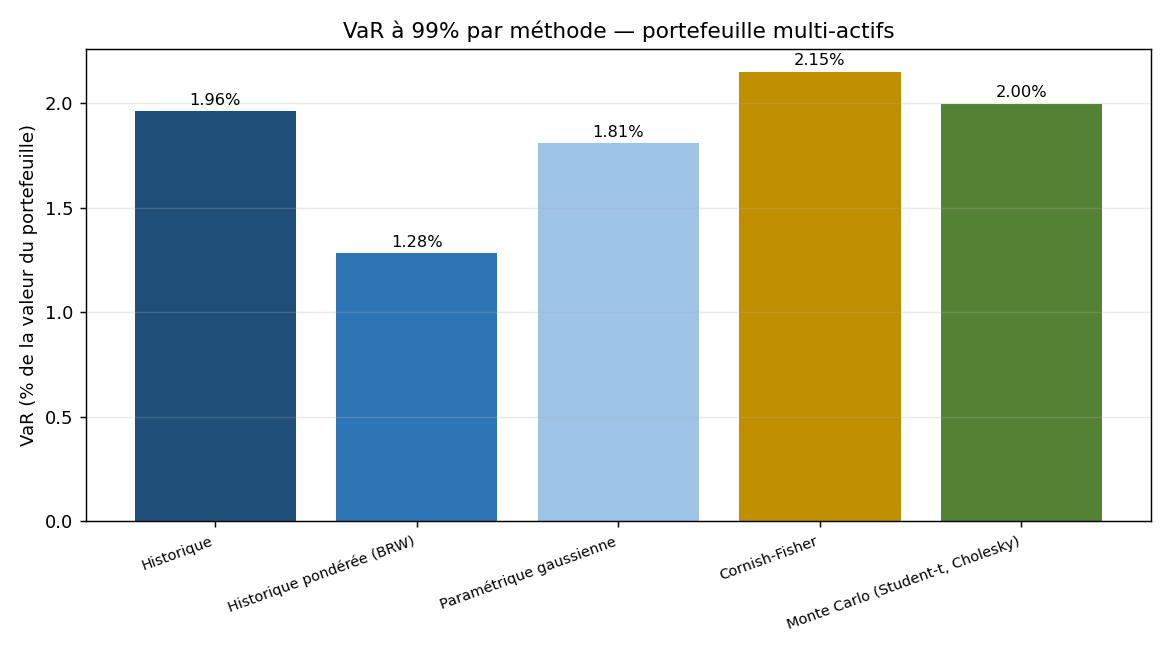
\includegraphics[width=0.78\textwidth]{../docs/img/01_var_methodes_comparaison.png}
\caption{One-day 99\% VaR by method (figure labels are in French).}
\end{figure}

\textbf{Backtest} (250 days, 500-day window): 4 breaches (1.6\% against 1\% expected).

\begin{center}
\begin{tabular}{@{}lcc@{}}
\toprule
Test & Statistic & $p$-value \\
\midrule
Kupiec POF & 0.7691 & 0.3805 \\
Christoffersen independence & 0.1306 & 0.7178 \\
Conditional coverage & 0.8998 & 0.6377 \\
\bottomrule
\end{tabular}
\end{center}
None of the tests rejects at 5\%. The traffic light is green (cumulative binomial probability 89.22\%, multiplier $3.00+0.00$).

\textbf{Stress tests} (P\&L in \% of portfolio value):

\begin{center}
\begin{tabular}{@{}lc@{}}
\toprule
Scenario & P\&L \\
\midrule
2008 replay & $-27.65\%$ \\
COVID, March 2020 & $-21.85\%$ \\
2022 rate shock & $-15.25\%$ \\
Hypothetical (equities $-25\%$, rates $+150$ bp, spreads $+120$ bp, USD $+8\%$) & $-16.60\%$ \\
\bottomrule
\end{tabular}
\end{center}
Forcing all correlations to 1 raises the annualised portfolio volatility from 12.54\% to 15.95\% ($+27.2\%$). The most plausible shock for a 15\% loss is mainly on equities: EU $-20.65\%$ and US $-26.31\%$, with credit at $-6.10\%$.

\textbf{Ex-ante tracking error.} The benchmark is 25\% EU equities, 25\% US equities, 25\% government bonds, 15\% credit and 10\% gold. Calibrated on 250 days, the forecast TE is 2.13\% against 1.68\% realised over the next 250 days (ratio 0.79). Over 48 rolling windows (step 21 days), the realised TE is on average 1.17 times the forecast. Raw beta is 1.173 and the Blume-adjusted beta is 1.115. The information ratio is 0.602. Equities account for 41.3\% (EU) and 52.6\% (US) of the normal VaR.

\section{Worked Example}
\textbf{Hypothetical scenario}, asset by asset. The sensitivities are the package defaults: sovereign bonds have a rate duration of 7, credit has a rate duration of 5 and a spread duration of 5, US equities carry full USD exposure and gold carries 0.3.
\begin{align*}
\text{EU equities}&: 0.30\times(-25\%) = -7.50\%\\
\text{US equities}&: 0.30\times(-25\%+1.0\times 8\%) = 0.30\times(-17\%) = -5.10\%\\
\text{Sovereign}&: 0.20\times(-7\times 0.0150) = 0.20\times(-10.5\%) = -2.10\%\\
\text{Credit}&: 0.15\times(-5\times 0.0150 - 5\times 0.0120) = 0.15\times(-13.5\%) = -2.025\%\\
\text{Gold}&: 0.05\times(0.3\times 8\%) = 0.05\times 2.4\% = +0.12\%
\end{align*}
The total is $-7.50-5.10-2.10-2.025+0.12=-16.605\%$, shown as $-16.60\%$ in the script output.

\textbf{Cornish-Fisher} with illustrative inputs: $\sigma=1\%$, $S=-0.5$, $K=3$, $\mu=0$, $z=-2.3263$.
\begin{align*}
z_{cf} &= -2.3263\;-0.3677\;-0.7014\;+0.0941 = -3.3013,\\
\mathrm{VaR}_{cf} &= 3.3013\times 1\% = 3.30\%\quad\text{against}\quad 2.33\%\ \text{for the normal VaR.}
\end{align*}

\textbf{Kupiec test} for the backtest above: $n=250$, $x=4$, $p=0.01$, $\hat p=0.016$.
\begin{align*}
\ln L_0 &= 246\ln 0.99+4\ln 0.01 = -2.4724-18.4207=-20.8931,\\
\ln L_1 &= 246\ln 0.984+4\ln 0.016 = -3.9678-16.5407=-20.5085,\\
LR_{uc} &= -2\,(-20.8931+20.5085)=0.7691\quad\Rightarrow\quad p\text{-value}=0.3805 .
\end{align*}

\section{Limits}
\begin{itemize}
\item \textbf{Synthetic data:} the historical scenario shocks are approximations of real crises, and the returns are simulated, so no conclusion applies to a real fund.
\item \textbf{Linear positions only:} there is no option gamma or vega.
\item \textbf{Normality in two places:} the parametric VaR and the Euler decomposition assume normal returns.
\item \textbf{Small backtest:} with 250 days and about 2.5 expected breaches, the tests have little power. A green zone is not proof that the model is right.
\item \textbf{One sample:} the tracking error ratios (0.79 and 1.17) come from one simulated path. These are model outputs, not recommendations.
\end{itemize}

\end{document}
